The figure \ref{figure:qresult} represents a typical output of the algorithm (the free parameters were $\sigma=0.1$, $C=2$, $K_1=10^{-2}$, $\alpha_{gap}=0.2$). One can see that corners, edges, small objects of the table are areas of high gradient norm. Among the keypoints one can visually distinguish three classes: sutuated at the corners of the objects (like corner of the monitor, keyboard, book), at the edges (for example the keyboard border is populated with keypoints) and in stable surface areas. The latter don't seem to be informative and probably should be supressed for the further applications.

Unfortunately the stability of keypoints was not perfect. The figure \ref{figure:vanish} illustrates a typical phenomenon of keypoint disappearance. The slight movement of sensor ($\approx$ 1cm) caused radical change of the gradient norm in the book corner. It stopped contain a local maximum of gradient norm which was a keypoint 0.03s ago. The figure also display support vectors in the area to emphasize the fact, that keypoint typically emerge in places with lots of support vectors. In \ref{figure:book012} one can see a dense cloud of support vectors in the book's corner, that is not there in \ref{figure:book015} anymore.

Finally, the found keypoints were frequently situated in the areas of unstable sufrace that potentially can complicate further descriptor calculations. The developers of NARF deliberately try to avoid such situation by explicit penalty \cite{steder2011point}. The further research is necessary to find out whether it is critical or not.

\begin{figure}
\centering
       \begin{subfigure}[b]{0.45\textwidth}
                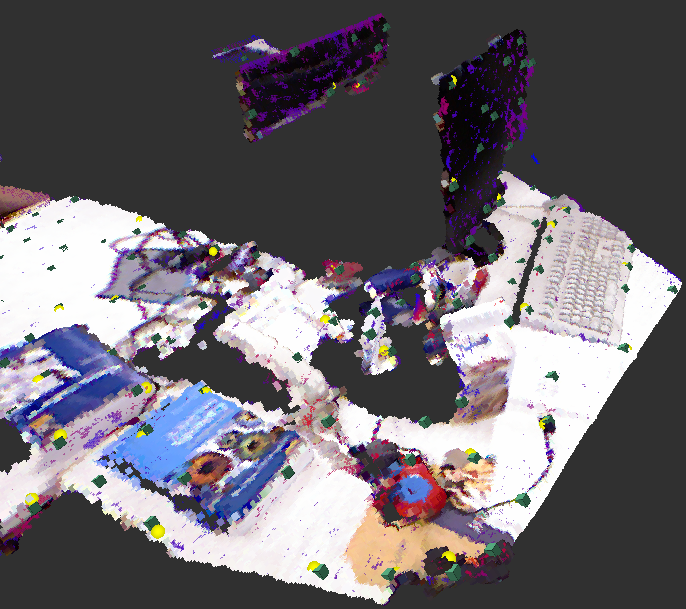
\includegraphics[width=\textwidth]{table018.png}
                \caption{RGB-D scan}
                \label{figure:rgbds}
       \end{subfigure}
       \begin{subfigure}[b]{0.45\textwidth}
                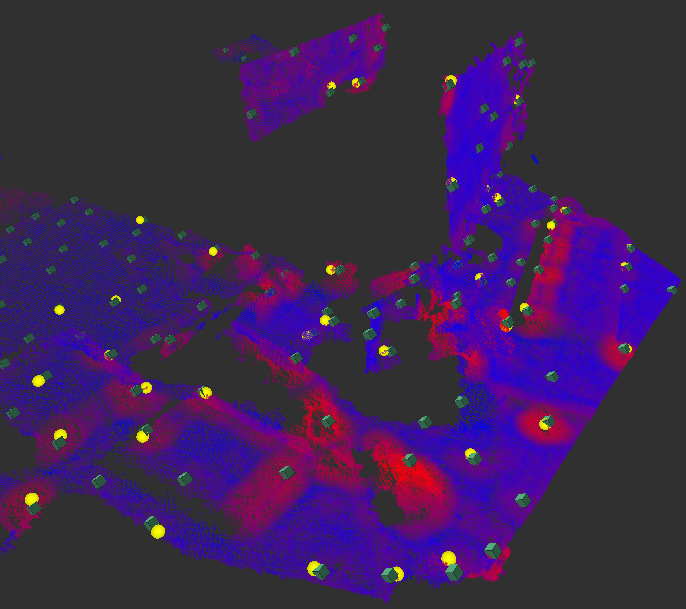
\includegraphics[width=\textwidth]{table018blue.png}
                \caption{Gradient norm map}
                \label{figure:gnm}
       \end{subfigure}
       \caption{Keypoint extraction result. The small green cubes on both pictures represent keypoints. The yellow spheres are keypoints from the previous scan that were sufficiently close (< 2cm) to the new ones. On the figure \ref{figure:gnm} the surface color represents the gradient norm: red denotes high and blue denotes low. A logarithmic transformation was used to map norm into color components.}
       \label{figure:qresult}
\end{figure}


\begin{figure}
\centering
       \begin{subfigure}[b]{0.45\textwidth}
                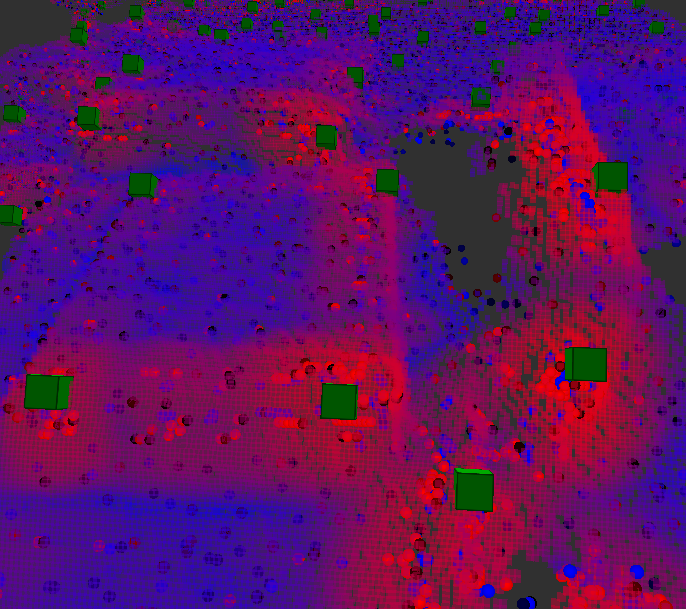
\includegraphics[width=\textwidth]{book12.png}
                \caption{At 0.12s from start}
                \label{figure:book012}
       \end{subfigure}
       \begin{subfigure}[b]{0.45\textwidth}
                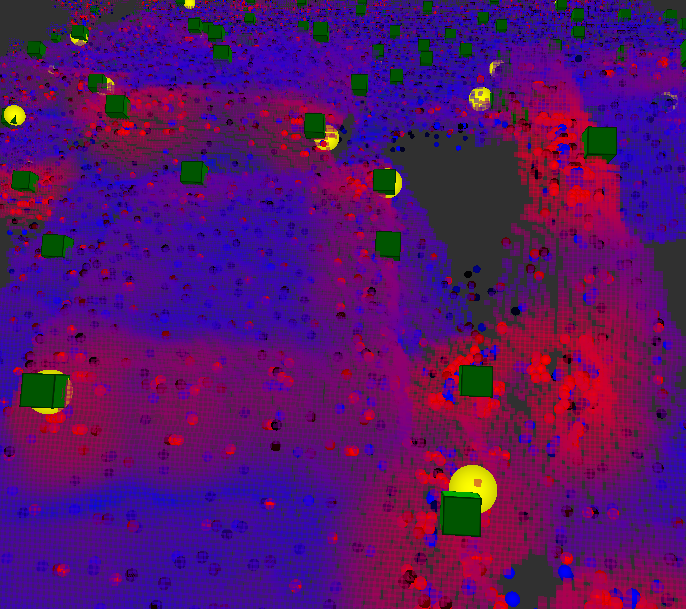
\includegraphics[width=\textwidth]{book15.png}
                \caption{At 0.15s from start}
                \label{figure:book015}
       \end{subfigure}
       \caption{The figure display keypoint vanishing. The close right corner of the book is a keypoint \ref{figure:book012} but stops being one on \ref{figure:book015}. For the explanation of markers and colors see \ref{figure:qresult}, additionally the support vectors are displayed in the same way as in \ref{fig:2books}}
        \label{figure:vanish}
\end{figure}